% =====================================================================
% AI Academy -- National AI Center
% Software Engineering Final Project -- Team Presentation Deck
% Based directly on SLIDES_TEMPLATE.tex supplied by the course.
% =====================================================================

\documentclass[aspectratio=169,11pt]{beamer}

% ===== CONFIGURATION =================================================
\newcommand{\teamname}{Team T1}
\newcommand{\topicchoice}{Food Analyzer}
\newcommand{\memberone}{Günəş Məmmədova}
\newcommand{\membertwo}{Esmira Məmmədova}
\newcommand{\memberthree}{Əli Muradov}
\newcommand{\memberfour}{Pünhan Mürsəlov}
\newcommand{\repolink}{github.com/Gunas12/Food\_Analyzer}

\newcommand{\coursecode}{AI-ENG-110}
\newcommand{\coursename}{Software Engineering}
\newcommand{\institution}{AI Academy, National AI Center}
\newcommand{\semester}{Spring 2026}

% ===== PACKAGES ======================================================
\usepackage{fontspec}
\setsansfont{Arial}
\setmonofont{Courier New}
\usepackage{xcolor}
\usepackage{tabularx}
\usepackage{booktabs}
\usepackage{listings}
\usepackage{tikz}
\usepackage{graphicx}
\usetikzlibrary{shapes.geometric,arrows.meta,positioning,fit,backgrounds}
\graphicspath{{../docs/screenshots/}{../data/}}

% ===== BEAMER THEME ==================================================
\usetheme{default}
\usefonttheme{professionalfonts}
\setbeamertemplate{navigation symbols}{}

\definecolor{accent}{HTML}{0B3D91}
\definecolor{accent2}{HTML}{8B0000}
\definecolor{soft}{HTML}{F2F4F8}
\definecolor{ok}{HTML}{166534}
\definecolor{warn}{HTML}{B45309}
\definecolor{ink}{HTML}{17212B}

\setbeamercolor{normal text}{fg=ink,bg=white}
\setbeamercolor{title}{fg=accent}
\setbeamercolor{frametitle}{fg=accent}
\setbeamercolor{section in head/foot}{bg=accent,fg=white}
\setbeamercolor{itemize item}{fg=accent}
\setbeamercolor{itemize subitem}{fg=accent}
\setbeamercolor{enumerate item}{fg=accent}
\setbeamercolor{block title}{bg=accent,fg=white}
\setbeamercolor{block body}{bg=soft,fg=black}

\setbeamerfont{title}{size=\Large,series=\bfseries}
\setbeamerfont{frametitle}{size=\large,series=\bfseries}
\setbeamerfont{footline}{size=\tiny}

\setbeamertemplate{footline}{%
  \leavevmode%
  \hbox to \paperwidth{\hspace*{2ex}\tiny\textit{\teamname{} -- \topicchoice}\hfill%
  \tiny\textit{\coursecode{} -- \semester{}}\hfill%
  \tiny\insertframenumber/\inserttotalframenumber\hspace*{2ex}}%
  \vskip1pt%
}

% ===== CODE LISTINGS =================================================
\definecolor{codegreen}{rgb}{0,0.45,0}
\definecolor{codepurple}{rgb}{0.48,0,0.66}
\lstdefinestyle{python}{
  language=Python,
  backgroundcolor=\color{soft},
  commentstyle=\color{codegreen},
  keywordstyle=\color{accent},
  stringstyle=\color{codepurple},
  basicstyle=\ttfamily\scriptsize,
  breaklines=true,
  frame=single,
  framerule=0.4pt,
  rulecolor=\color{black!30},
  showstringspaces=false,
}
\newcommand{\source}[1]{\vfill\hfill{\tiny\color{black!55}Source: \texttt{\detokenize{#1}}}}

% =====================================================================
\begin{document}

% ========== SLIDE 1: TITLE ===========================================
{%
\setbeamertemplate{footline}{}
\begin{frame}[plain]
  \begin{center}
    \vspace{0.45cm}
    {\small \textsc{\institution}}\\[0.2em]
    {\small \textsc{\coursecode{} -- \coursename{} -- \semester{}}}\\[1em]
    \rule{0.72\textwidth}{0.6pt}\\[0.35em]
    {\Huge\bfseries\color{accent} Food Analyzer}\\[0.25em]
    {\large Image-to-Nutrition Analysis}\\[0.35em]
    \rule{0.72\textwidth}{0.6pt}\\[0.9em]
    {\large \teamname}\\[0.45em]
    {\normalsize \memberone\quad\textbullet\quad\membertwo}\\[0.2em]
    {\normalsize \memberthree\quad\textbullet\quad\memberfour}\\[0.75em]
    {\footnotesize\itshape Final Project Defense -- September 2026}\\[0.25em]
    {\footnotesize\texttt{\repolink}}
  \end{center}
  \note{Layihənin məqsədini bir cümlə ilə təqdim edin: şəkildən yeməyi və ingredientləri tanıyıb strukturlaşdırılmış nutrition nəticəsi yaratmaq.}
\end{frame}
}

% ========== SLIDE 2: PROBLEM + CONTRACT ==============================
\begin{frame}{The problem and system contract}
  \begin{block}{What the system does}
    A user submits a meal image; the system identifies ingredients, scales nutrition facts to estimated portions, and stores a structured analysis record.
  \end{block}

  \begin{columns}[T,onlytextwidth]
  \column{0.48\textwidth}
  \textbf{Input}
  \begin{itemize}\setlength\itemsep{0.25em}
    \item JPEG or PNG image
    \item Maximum upload size: 5 MB
    \item Content type and magic bytes must agree
  \end{itemize}

  \column{0.48\textwidth}
  \textbf{Output}
  \begin{itemize}\setlength\itemsep{0.25em}
    \item Recognition status and ingredient rows
    \item Calories, protein, carbs, and fat
    \item Database id, image path, and timestamp
  \end{itemize}
  \end{columns}

  \textbf{Entry points:} FastAPI web/API interface and command-line interface.
  \source{README.md; src/api.py; src/models.py}
  \note{Input və output sərhədlərini izah edin. Sistem tibbi və ya laboratoriya dəqiqliyi iddiası etmir; nəticə provider-lərin verdiyi təxminlərə əsaslanır.}
\end{frame}

% ========== SLIDE 3: REQUEST LIFECYCLE ===============================
\begin{frame}{Request lifecycle}
  \begin{center}
  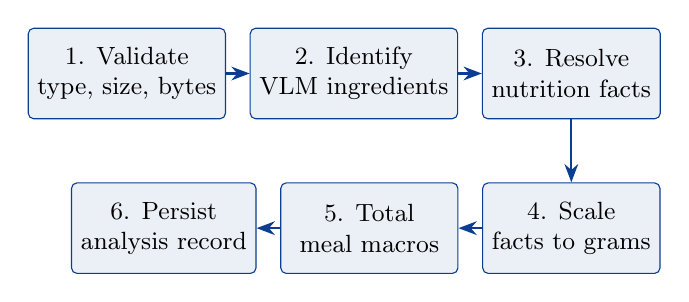
\begin{tikzpicture}[
    node distance=3mm,
    stage/.style={draw=accent,fill=accent!8,rounded corners=2pt,minimum width=2.25cm,minimum height=1.15cm,align=center,font=\small},
    arrow/.style={-Stealth,thick,draw=accent}
  ]
    \node[stage] (v) {1. Validate\\type, size, bytes};
    \node[stage,right=of v] (i) {2. Identify\\VLM ingredients};
    \node[stage,right=of i] (r) {3. Resolve\\nutrition facts};
    \node[stage,below=8mm of r] (s) {4. Scale\\facts to grams};
    \node[stage,left=of s] (t) {5. Total\\meal macros};
    \node[stage,left=of t] (p) {6. Persist\\analysis record};
    \draw[arrow] (v) -- (i);
    \draw[arrow] (i) -- (r);
    \draw[arrow] (r) -- (s);
    \draw[arrow] (s) -- (t);
    \draw[arrow] (t) -- (p);
  \end{tikzpicture}
  \end{center}

  \vspace{0.3em}
  \begin{columns}[T,onlytextwidth]
  \column{0.32\textwidth}
  \textbf{Invalid image}\par
  Stops before any provider call.
  \column{0.32\textwidth}
  \textbf{No meal detected}\par
  Returns a normal empty record.
  \column{0.32\textwidth}
  \textbf{Partial lookup failure}\par
  Preserves successful ingredients.
  \end{columns}
  \source{docs/architecture.md; src/core/analyzer.py}
  \note{Altı mərhələni ardıcıl izah edin. Xüsusilə validation provider çağırışından əvvəl işləyir və partial nutrition failure bütün nəticəni itirmir.}
\end{frame}

% ========== SLIDE 4: ARCHITECTURE ====================================
\begin{frame}{Architecture}
  \textbf{The supplied \texttt{ai/} package is isolated behind our software-engineering layer.}

  \vspace{0.35em}
  \begin{center}
  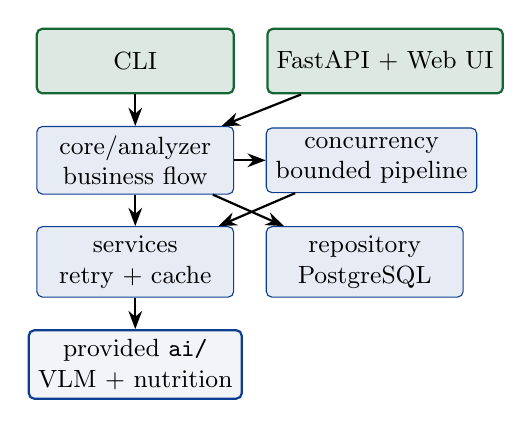
\begin{tikzpicture}[
    node distance=4mm,
    box/.style={draw,rounded corners=2pt,minimum width=2.5cm,minimum height=0.82cm,align=center,font=\small},
    aibox/.style={box,fill=soft,draw=accent,thick},
    sebox/.style={box,fill=accent!10,draw=accent},
    entry/.style={box,fill=ok!15,draw=ok,thick},
    arrow/.style={-Stealth,thick}
  ]
    \node[entry] (cli) {CLI};
    \node[entry,right=of cli] (api) {FastAPI + Web UI};
    \node[sebox,below=of cli] (core) {core/analyzer\\business flow};
    \node[sebox,right=of core] (conc) {concurrency\\bounded pipeline};
    \node[sebox,below=of core] (svc) {services\\retry + cache};
    \node[sebox,right=of svc] (store) {repository\\PostgreSQL};
    \node[aibox,below=of svc] (ai) {provided \texttt{ai/}\\VLM + nutrition};
    \draw[arrow] (cli) -- (core);
    \draw[arrow] (api) -- (core);
    \draw[arrow] (core) -- (conc);
    \draw[arrow] (core) -- (svc);
    \draw[arrow] (conc) -- (svc);
    \draw[arrow] (svc) -- (ai);
    \draw[arrow] (core) -- (store);
  \end{tikzpicture}
  \end{center}

  \textbf{Consequence:} provider implementations can change while application models and tests remain stable.
  \source{docs/architecture.md; src/; ai/}
  \note{Bu diagram dependency boundary-ni göstərir. Entry point-lər core-a daxil olur, core isə provider və storage detalları ilə abstraction-lar vasitəsilə işləyir.}
\end{frame}

% ========== SLIDE 5: DESIGN DECISIONS ================================
\begin{frame}{Three design decisions we can defend}
  \begin{enumerate}\setlength\itemsep{0.55em}
    \item \textbf{Async orchestration with thread offloading}\
      Provider SDK calls are synchronous, so \texttt{asyncio.to\_thread} keeps the event loop responsive.
    \item \textbf{Bounded concurrency instead of unlimited fan-out}\
      A semaphore limits simultaneous nutrition lookups and protects external providers.
    \item \textbf{Shared response builder for API and CLI}\
      One implementation scales portions and totals, preventing interface-specific calculation drift.
  \end{enumerate}

  \begin{block}{Accepted trade-off}
    The cache and semaphore are process-local. Horizontal scaling requires a shared limiter and shared cache.
  \end{block}
  \source{src/services/ai_service.py; src/concurrency/pipeline.py; src/core/lines.py}
  \note{Hər qərar üçün alternativi qısa qeyd edin: blocking call, unbounded gather və duplicate calculation logic. Sonra niyə seçilən yanaşmanın daha təhlükəsiz olduğunu izah edin.}
\end{frame}

% ========== SLIDE 6: WEB INTERFACE ===================================
\begin{frame}{Browser interface as a thin client}
  \begin{columns}[T,onlytextwidth]
  \column{0.58\textwidth}
    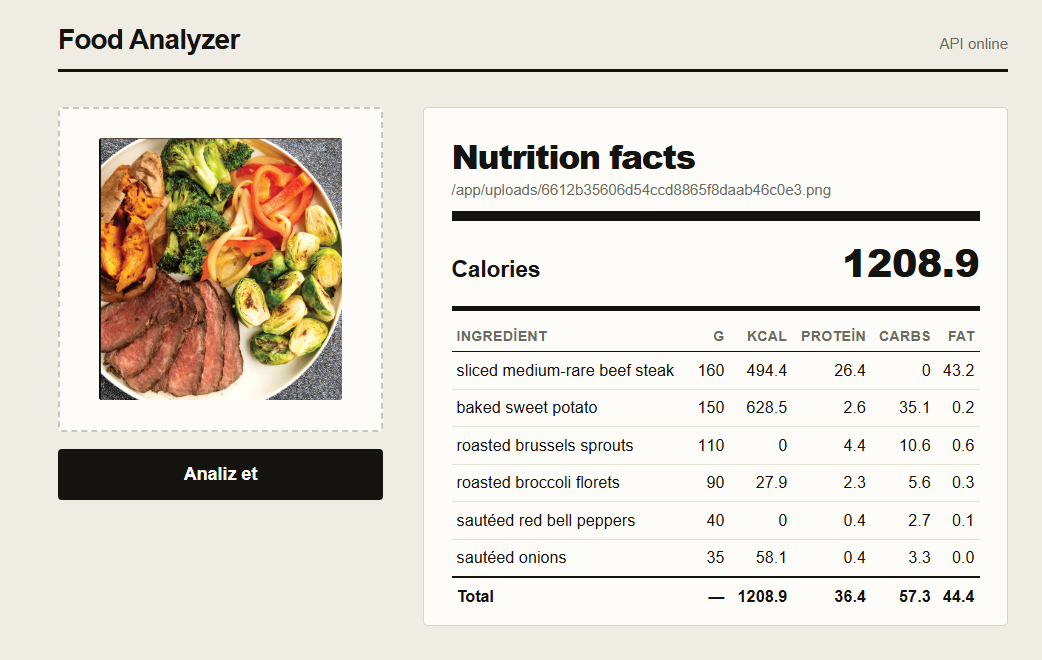
\includegraphics[width=\linewidth,height=0.70\textheight,keepaspectratio]{web-ui.png}
  \column{0.39\textwidth}
    \textbf{The browser is responsible for}
    \begin{itemize}\setlength\itemsep{0.35em}
      \item selecting and submitting an image;
      \item rendering ingredient rows and totals;
      \item displaying API validation or provider errors.
    \end{itemize}
    \begin{block}{Boundary}
      Nutrition calculations remain in the application layer, not in JavaScript.
    \end{block}
  \end{columns}
  \source{static/index.html; docs/screenshots/web-ui.png}
  \note{UI-nin yalnız client olduğunu vurğulayın. Business logic server-də qalır, buna görə CLI və HTTP eyni nəticə modelindən istifadə edir.}
\end{frame}

% ========== SLIDE 7: HTTP API ========================================
\begin{frame}{HTTP API contract}
  \begin{columns}[T,onlytextwidth]
  \column{0.58\textwidth}
  \scriptsize
  \setlength{\tabcolsep}{4pt}
  \begin{tabular}{@{}llll@{}}
    \toprule
    \textbf{Method} & \textbf{Route} & \textbf{Success} & \textbf{Failure} \\
    \midrule
    GET  & / & Web UI & 404 \\
    GET  & /health & status: ok & 503 \\
    POST & /analyze & AnalysisRecord & 400/503 \\
    GET  & /analyses/:id & AnalysisRecord & 404 \\
    \bottomrule
  \end{tabular}

  \vspace{0.5em}
  \textbf{Contract detail}\par
  \footnotesize\texttt{POST /analyze} accepts multipart field \texttt{file}. A recognized=false result is valid HTTP 200 data, not an exception.

  \column{0.38\textwidth}
    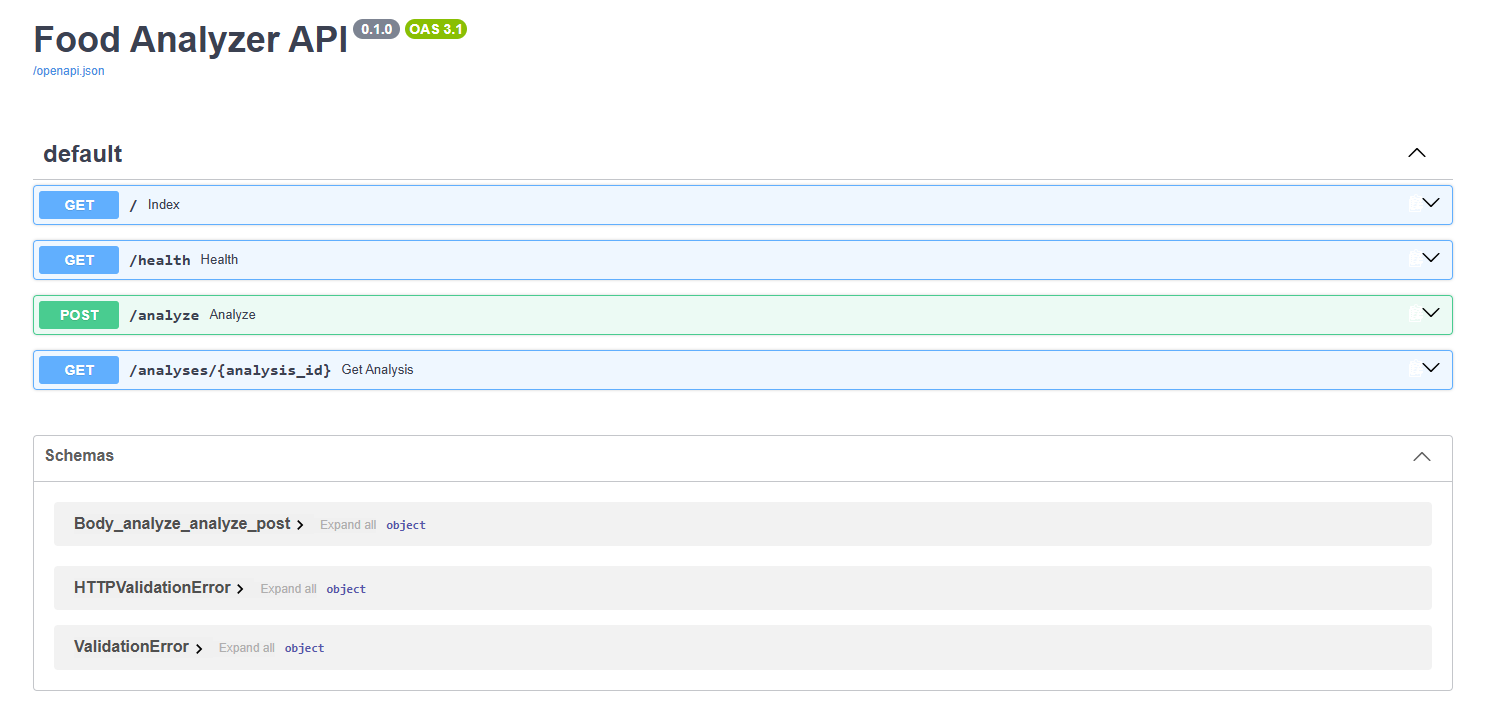
\includegraphics[width=\linewidth,height=0.62\textheight,keepaspectratio]{swagger-docs.png}
  \end{columns}
  \source{src/api.py; docs/api.md}
  \note{Dörd route-u izah edin. 400 client upload xətasıdır, 503 provider və ya service problemidir, recognized=false isə normal nəticədir.}
\end{frame}

% ========== SLIDE 8: VALIDATION ======================================
\begin{frame}[fragile]{Upload validation and path safety}
  \begin{columns}[T,onlytextwidth]
  \column{0.60\textwidth}
  \begin{lstlisting}[style=python]
content = await file.read()
if len(content) > MAX_UPLOAD_BYTES:
    raise HTTPException(400, "File exceeds the limit")

if not has_image_magic_bytes(content[:16]):
    raise HTTPException(400, "Invalid image")

safe_name = f"{uuid.uuid4()}{suffix}"
path = (UPLOAD_DIR / safe_name).resolve()
if UPLOAD_DIR.resolve() not in path.parents:
    raise HTTPException(400, "Unsafe path")
  \end{lstlisting}
  \column{0.36\textwidth}
  \textbf{Three checks}
  \begin{enumerate}\setlength\itemsep{0.35em}
    \item Content type and extension
    \item JPEG/PNG magic bytes
    \item Server-generated UUID path
  \end{enumerate}
  \begin{block}{Security result}
    A client filename never becomes a trusted filesystem path.
  \end{block}
  \end{columns}
  \source{src/api.py; src/validation.py}
  \note{Validation-un yalnız extension-a güvənmədiyini göstərin. Magic bytes fayl məzmununu yoxlayır, UUID isə path traversal riskini azaldır.}
\end{frame}

% ========== SLIDE 9: RESPONSE CONSTRUCTION ===========================
\begin{frame}[fragile]{Response construction and nutrition scaling}
  \begin{columns}[T,onlytextwidth]
  \column{0.57\textwidth}
  \begin{lstlisting}[style=python]
facts = facts_by_name.get(ingredient.name)
if facts is None:
    lines.append(IngredientLine(
        name=ingredient.name,
        estimated_grams=ingredient.estimated_grams,
        kcal=0.0, protein_g=0.0,
        carbs_g=0.0, fat_g=0.0,
    ))
    continue

portion = facts.for_grams(ingredient.estimated_grams)
totals = compute_totals(ingredients, facts_by_name)
  \end{lstlisting}
  \column{0.39\textwidth}
  \textbf{Calculation rule}
  \begin{itemize}\setlength\itemsep{0.35em}
    \item Provider facts are per 100 g.
    \item Each row is scaled to the estimated portion.
    \item The supplied totals function calculates meal totals.
  \end{itemize}
  \begin{block}{Partial result policy}
    A missing lookup remains visible with zero macros.
  \end{block}
  \end{columns}
  \source{src/core/lines.py}
  \note{Provider-in məlumatı 100 qram üçündür. Builder estimated grams əsasında porsiyanı hesablayır. Lookup alınmadıqda ingredient itmir, amma macro-lar sıfır göstərilir.}
\end{frame}

% ========== SLIDE 10: DEPLOYMENT =====================================
\begin{frame}{Container and deployment topology}
  \begin{center}
  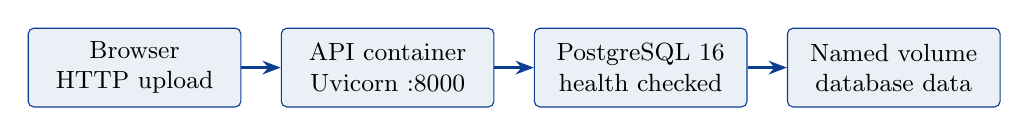
\begin{tikzpicture}[
    node distance=5mm,
    box/.style={draw=accent,fill=accent!8,rounded corners=2pt,minimum width=2.7cm,minimum height=1cm,align=center,font=\small},
    arrow/.style={-Stealth,thick,draw=accent}
  ]
    \node[box] (browser) {Browser\\HTTP upload};
    \node[box,right=of browser] (api) {API container\\Uvicorn :8000};
    \node[box,right=of api] (db) {PostgreSQL 16\\health checked};
    \node[box,right=of db] (vol) {Named volume\\database data};
    \draw[arrow] (browser) -- (api);
    \draw[arrow] (api) -- (db);
    \draw[arrow] (db) -- (vol);
  \end{tikzpicture}
  \end{center}

  \begin{columns}[T,onlytextwidth]
  \column{0.48\textwidth}
  \textbf{Runtime controls}
  \begin{itemize}
    \item Python 3.12 slim image
    \item Non-root application user
    \item Database readiness check
  \end{itemize}
  \column{0.48\textwidth}
  \textbf{Known deployment boundary}
  \begin{itemize}
    \item Database data is persistent
    \item Uploaded images use local container storage
  \end{itemize}
  \end{columns}
  \source{Dockerfile; docker-compose.yml}
  \note{Container axınını soldan sağa izah edin. Database üçün named volume var, amma upload faylları ayrıca persistent volume-a bağlanmayıb.}
\end{frame}

% ========== SLIDE 11: ASYNC BOUNDARY =================================
\begin{frame}[fragile]{Synchronous providers inside an async application}
  \begin{columns}[T,onlytextwidth]
  \column{0.58\textwidth}
  \begin{lstlisting}[style=python]
async def _call_with_retry(self, call, operation):
    attempt = 0
    while True:
        try:
            result = await asyncio.to_thread(call)
            return result
        except ProviderError:
            attempt += 1
            if attempt >= self.max_attempts:
                raise
            await asyncio.sleep(self.base_delay * attempt)
  \end{lstlisting}
  \column{0.38\textwidth}
  \textbf{Execution model}
  \begin{itemize}\setlength\itemsep{0.35em}
    \item Event loop schedules requests.
    \item Worker thread runs blocking SDK code.
    \item Await resumes when the call finishes.
  \end{itemize}
  \begin{block}{Why it matters}
    One slow provider call does not freeze unrelated requests.
  \end{block}
  \end{columns}
  \source{src/services/ai_service.py}
  \note{asyncio.to_thread-in məqsədi provider SDK-nın blocking call-unu event loop-dan çıxarmaqdır. Bu, digər request-lərin işləməsinə imkan verir.}
\end{frame}

% ========== SLIDE 12: RETRY POLICY ===================================
\begin{frame}{Retry policy and error discipline}
  \begin{center}
  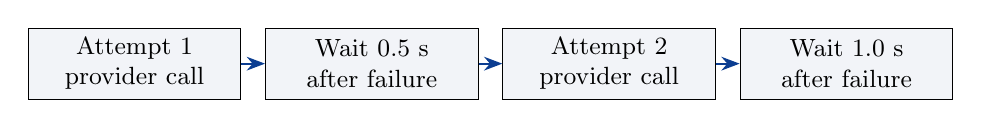
\begin{tikzpicture}[
    node distance=3mm,
    retrybox/.style={draw,fill=soft,minimum width=2.7cm,minimum height=0.9cm,align=center,font=\small},
    arrow/.style={-Stealth,thick,draw=accent}
  ]
    \node[retrybox] (a1) {Attempt 1\\provider call};
    \node[retrybox,right=of a1] (w1) {Wait 0.5 s\\after failure};
    \node[retrybox,right=of w1] (a2) {Attempt 2\\provider call};
    \node[retrybox,right=of a2] (w2) {Wait 1.0 s\\after failure};
    \draw[arrow] (a1) -- (w1);
    \draw[arrow] (w1) -- (a2);
    \draw[arrow] (a2) -- (w2);
  \end{tikzpicture}
  \end{center}

  \begin{columns}[T,onlytextwidth]
  \column{0.48\textwidth}
  \textbf{Retry only transient boundaries}
  \begin{itemize}
    \item Maximum 3 attempts
    \item Linear backoff: 0.5 s, then 1.0 s
    \item Only \texttt{ProviderError} is retried
  \end{itemize}
  \column{0.48\textwidth}
  \textbf{Keep programming errors visible}
  \begin{itemize}
    \item Validation failures return immediately
    \item Unexpected exceptions are not converted into retries
    \item Logs avoid raw provider payloads
  \end{itemize}
  \end{columns}
  \source{src/services/ai_service.py; tests/test_ai_service.py}
  \note{Retry-nin yalnız ProviderError üçün işlədiyini vurğulayın. Bu, programming error-ları gizlətmir və problem olduqda səbəbi tapmağı asanlaşdırır.}
\end{frame}

% ========== SLIDE 13: CACHE ==========================================
\begin{frame}[fragile]{TTL cache invariants}
  \begin{columns}[T,onlytextwidth]
  \column{0.56\textwidth}
  \begin{lstlisting}[style=python]
key = name.strip().casefold()
with self._lock:
    entry = self._entries.get(key)
    if entry is None:
        return None
    facts, expires_at = entry
    if self._clock() >= expires_at:
        del self._entries[key]
        return None
    return facts
  \end{lstlisting}
  \column{0.40\textwidth}
  \textbf{Stable key}\par
  ``Rice'' and ``rice'' share one entry.\\[0.55em]
  \textbf{Stable clock}\par
  Monotonic time prevents expiry errors when the system clock changes.\\[0.55em]
  \textbf{Thread safety}\par
  A lock protects the dictionary used by worker threads.
  \end{columns}
  \begin{block}{Scope}
    Default TTL: 86,400 seconds. Cache scope: one application process.
  \end{block}
  \source{src/services/nutrition_cache.py}
  \note{Cache key normalization, monotonic clock və lock üç əsas invariant-dır. Cache process-local olduğuna görə multi-container deployment-da paylaşılmır.}
\end{frame}

% ========== SLIDE 14: PARALLEL PIPELINE ==============================
\begin{frame}[fragile]{Bounded parallel nutrition pipeline}
  \begin{columns}[T,onlytextwidth]
  \column{0.58\textwidth}
  \begin{lstlisting}[style=python]
groups = list(group_by_key(items))
results = await asyncio.gather(*(
    self._lookup_group(key, group)
    for key, group in groups
))

async with self._semaphore:
    facts = self.cache.get(name)  # recheck
    if facts is None:
        facts = await self.ai.nutrition(name)
        self.cache.set(name, facts)
  \end{lstlisting}
  \column{0.38\textwidth}
  \textbf{Pipeline properties}
  \begin{itemize}\setlength\itemsep{0.3em}
    \item Deduplicate normalized ingredient names
    \item Bound simultaneous provider calls
    \item Recheck cache after waiting for a slot
    \item Preserve successful partial results
  \end{itemize}
  \end{columns}
  \source{src/concurrency/pipeline.py}
  \note{Eyni ingredient təkrar gəlsə bir lookup edilir. Semaphore provider yükünü məhdudlaşdırır. Slot gözlədikdən sonra cache yenidən yoxlanır ki, başqa task-ın nəticəsi təkrar çağırış yaratmasın.}
\end{frame}

% ========== SLIDE 15: BENCHMARK ======================================
\begin{frame}{Concurrency: the benchmark}
  \textbf{Workload:} ten nutrition lookups with 150 ms synthetic provider latency.

  \vspace{0.45em}
  \begin{center}
  \begin{tabular}{lcc}
    \toprule
    & \textbf{Sequential} & \textbf{Concurrent} \\
    \midrule
    Wall-clock (s) & 1.517 & 0.154 \\
    Speedup & 1.0$\times$ & \textbf{9.9$\times$} \\
    Lookup count & 10 & 10 \\
    \bottomrule
  \end{tabular}
  \end{center}

  \vspace{0.5em}
  \begin{block}{Interpretation}
    Independent I/O-bound lookups overlap while the semaphore defines the maximum provider pressure.
  \end{block}
  \textbf{What this does not prove:} the provider is fake, so the result demonstrates pipeline overhead rather than a production latency or SLA.
  \source{artefacts/benchmark.txt; scripts/benchmark.py}
  \note{Rəqəmləri dəqiq deyin: 1.517 saniyədən 0.154 saniyəyə, 9.9 dəfə sürətlənmə. Bunun synthetic benchmark olduğunu və production SLA olmadığını qeyd edin.}
\end{frame}

% ========== SLIDE 16: PERSISTENCE ====================================
\begin{frame}[fragile]{Async repository and data model}
  \begin{columns}[T,onlytextwidth]
  \column{0.56\textwidth}
  \begin{lstlisting}[style=python]
async def save(self, record: AnalysisRecord):
    async with self._session() as session:
        row = AnalysisRecordModel(
            image_path=record.image_path,
            meal_recognized=record.meal_recognized,
            ingredients=[x.model_dump() for x in record.ingredients],
            totals=record.totals.model_dump(),
        )
        session.add(row)
        await session.commit()
        await session.refresh(row)
        return self._to_record(row)
  \end{lstlisting}
  \column{0.40\textwidth}
  \textbf{Model layers}
  \begin{itemize}\setlength\itemsep{0.3em}
    \item \texttt{IngredientLine}: one displayed ingredient
    \item \texttt{MealTotals}: meal summary
    \item \texttt{AnalysisRecord}: persisted public result
    \item SQLAlchemy model: JSON ingredients and totals
  \end{itemize}
  \begin{block}{Trade-off}
    JSON preserves the response shape but weakens relational ingredient queries.
  \end{block}
  \end{columns}
  \source{src/models.py; src/storage/repository.py}
  \note{Repository database detallarını core logic-dən ayırır. JSON sütunları nested response-u rahat saxlayır, amma ingredient üzrə relational sorğuları çətinləşdirir.}
\end{frame}

% ========== SLIDE 17: TESTING ========================================
\begin{frame}{Testing and saved evidence}
  \begin{columns}[T,onlytextwidth]
  \column{0.38\textwidth}
    {\fontsize{28}{32}\selectfont\bfseries\color{accent}143 / 143}\par
    {\small\color{ok}\textbf{tests passed in the saved run}}\\[1em]
    {\fontsize{28}{32}\selectfont\bfseries\color{accent}97\%}\par
    {\small\color{ok}\textbf{saved source coverage}}
  \column{0.58\textwidth}
    \textbf{Tests worth calling out}
    \begin{itemize}\setlength\itemsep{0.35em}
      \item Event gates prove concurrent overlap without fragile sleeps.
      \item Fake VLM and nutrition providers keep the suite offline.
      \item API tests cover upload limits, magic bytes, and error mapping.
      \item Repository tests verify model-to-row round trips.
    \end{itemize}
    \begin{block}{Saved environment}
      Python 3.13.15 -- pytest 9.1.1 -- 143 passed in 3.40 s.
    \end{block}
  \end{columns}
  \source{artefacts/coverage.txt; tests/}
  \note{Bu rəqəmlərin artefact-da saxlanmış run olduğunu deyin. Testlər external network və API key tələb etmir. Concurrency event gate ilə yoxlanır.}
\end{frame}

% ========== SLIDE 18: LIMITATIONS ====================================
\begin{frame}{Limitations and what we would do next}
  \begin{columns}[T,onlytextwidth]
  \column{0.48\textwidth}
  \textbf{Where the system is brittle today}
  \begin{itemize}\setlength\itemsep{0.35em}
    \item No explicit timeout around provider calls
    \item Semaphore is local to each pipeline instance
    \item Cache is in-memory and process-local
    \item Uploaded images use local container storage
    \item No HTTP route for listing recent analyses
  \end{itemize}
  \column{0.48\textwidth}
  \textbf{Given another week we would}
  \begin{enumerate}\setlength\itemsep{0.35em}
    \item Add a service timeout and shared provider limiter
    \item Move cache state to Redis for horizontal scaling
    \item Persist uploads in object storage or a volume
    \item Expose recent history through the repository contract
    \item Add load tests and distributed traces
  \end{enumerate}
  \end{columns}
  \source{docs/architecture.md; Dockerfile; docker-compose.yml}
  \note{Limitations-i müdafiə olunan şəkildə təqdim edin: bunlar gizli problem deyil, mövcud scope-un sərhədləridir. Prioritet service timeout və process-wide provider limiter-dir.}
\end{frame}

% ========== SLIDE 19: TEAM CONTRIBUTIONS =============================
\begin{frame}{Team contributions and AI disclosure}
  \begin{center}\small
  \begin{tabularx}{\linewidth}{lXr}
    \toprule
    \textbf{Member} & \textbf{Primary contribution areas} & \textbf{Commits} \\
    \midrule
    \memberone & Models, wiring, CLI, Docker, validation, documentation & 14 \\
    \membertwo & FastAPI, web UI, benchmark, shared response logic & 12 \\
    \memberthree & Retry service, TTL cache, concurrent pipeline, tests & 4 \\
    \memberfour & Async repository, persistence tests, storage dependencies & 6 \\
    \bottomrule
  \end{tabularx}
  \end{center}

  \begin{block}{Shared ownership}
    The team reviewed the complete system and can explain the request flow, failure model, and trade-offs across module boundaries.
  \end{block}

  \textbf{AI tool use:} AI assistants supported planning, drafting, debugging, and review. Team members reviewed the generated changes, ran the available checks, and remain responsible for the final technical decisions.
  \source{Git contribution history; report/CONTRIBUTION_STATEMENT.md}
  \note{Contribution cədvəlini qısa izah edin. AI disclosure-u açıq deyin: AI kömək edib, amma qərarlar, review və nəticənin məsuliyyəti komandadadır.}
\end{frame}

% ========== SLIDE 20: Q&A ============================================
{%
\setbeamertemplate{footline}{}
\begin{frame}[plain]
  \begin{center}
    \vspace{0.75cm}
    {\Huge\bfseries\color{accent} Questions?}\\[1em]
    \rule{0.55\textwidth}{0.6pt}\\[1em]
    {\large \teamname}\\[0.45em]
    {\normalsize \memberone\quad\textbullet\quad\membertwo}\\[0.2em]
    {\normalsize \memberthree\quad\textbullet\quad\memberfour}\\[0.75em]
    {\normalsize \texttt{\repolink}}\\[0.8em]
    {\footnotesize\itshape ``We can walk through any file in the repository.''}
  \end{center}
  \note{Suallar üçün sözü auditoriyaya verin. Lazım olsa architecture, benchmark və ya validation kodunu açmağa hazır olun.}
\end{frame}
}

\end{document}
